\chapter{Relative constructions} \label{ch:relatives}
\is{relative construction|(}\is{relative clause|(}\is{gap, gapping!in relative clauses|(}\is{supplement vs modifier|(}

\epigraph{That which binds us\\
is not the thing itself\\
but the space where\\
it should have been.}{}

\section{Introduction}
\is{subordinator!\textit{that} (relative)}\is{preposition, preposition phrase (PP)!as subject}\is{anaphora!antecedent–gap relation}

The following (paraphrased) \href{https://www.reddit.com/r/EnglishLearning/comments/1b03e2u/relative_pronouns_i_wouldnt_like_to_stay_in_a/}{question from Reddit/EnglishLearning} is a good illustration of the confusion that often swirls around relative constructions.

\begin{quote}
    Can I use \textit{where} instead of \textit{that} in the relative clause in \textit{I wouldn't like to stay in a hotel \uline{that doesn't have air conditioning}.} It seems that, if \textit{where} is used for places and a hotel is a place, then this should be possible. But it sounds ungrammatical.
\end{quote}

Indeed it is ungrammatical, and although \textit{where} certainly denotes places (along with situations, academic areas, etc.), we can't rely on semantics here. Once again, we need to look at the syntax.

A \textsc{relative clause} is ``relative'' because of an anaphoric \strong{relationship} between it and the main clause. If we make the two independent, we get (\ref{ex:two-sentence-version}a) along with (b) but not (c).

\ea\label{ex:two-sentence-version}
    \ea[]{\textit{I wouldn't like to stay in \uline{a hotel}.}}
    \ex[]{\textit{\uline{It} doesn't have air conditioning.}}
    \ex[*]{\textit{\uline{There} doesn't have air conditioning.}}
    \z
\z

The relationship here is that between \textit{hotel} in (\ref{ex:two-sentence-version}a) and the pronoun \textit{it} in (b). And the reason you can't use the preposition \textit{where} in the relative clause is the same reason that you can't use \textit{there} in the independent clause: because most clauses resist PP subjects. Instead we end up with (\ref{ex:no-it}).

\ea[]{\textit{I wouldn't like to stay in a hotel \uline{that }}\uline{[it] }\textit{\uline{doesn't have air conditioning}.}}\label{ex:no-it}
\z

This illustrates a key property of the relative clause: \textit{It} does not actually appear. Instead there is a gap where the subject should be.\is{subject (Subj)!gap position} To generalize, whatever anaphor would typically appear in an independent clause is replaced by a gap in its relative counterpart. The gap in (\ref{ex:no-it}) happens to be the subject, but in other relative clauses, it could be an adjunct, object, or other complement, as in (\ref{ex:articulated-gap-positions}). This gapping behaviour should remind you of focused interrogatives, which leave a gap wherever the focused element would usually appear in a ``normal'' clause.\is{interrogative clause!focused vs relative}

\ea \label{ex:articulated-gap-positions}
    \ea[]{\textit{That's the kid \ob who \uline{\phantom{he}} arrived yesterday \cb.}\hfill[\textsc{subject}]}
    \ex[]{\textit{The point \ob which I raised \uline{\phantom{it}} \cb~was shot down.}\hfill[\textsc{object}]}
    \ex[]{\textit{That's the place \ob where I put it \uline{\phantom{there}} \cb.}\hfill[\textsc{complement}]}
    \ex[]{\textit{That's the year \ob when we won the cup \uline{\phantom{then}} \cb.}\hfill[\textsc{modifier}]}
    \z
\z
\is{relative word|(}

\section{Syntactic types}
\is{relative clause!types}\is{relative clause!basic|(}\is{relative clause!that@\textit{that}}\is{relative clause!bare}

If you've heard anything at all about relative clauses, it's probably that ``restrictive relatives'' start with \textit{that} and ``non-restrictive relatives'' start with \textit{which}. Unfortunately, this factoid is rather unhelpful.

A clearer way to think about it is set out in Figure \ref{fig:relative-construction-types}. We can say that English relative clauses come in two broad syntactic types: basic and focused. The basic ones can be subdivided into \textit{that}-marked and bare relatives, while the focused types can be subdivided into articulated, infinitival, and fused relatives.\is{articulated relative}\is{infinitival!relative}\is{fused relative} Examples follow in (\ref{ex:basic-rel-clause-types} \& \ref{ex:focused-rel-clause-types}).

\begin{figure}[ht]
    \centering
    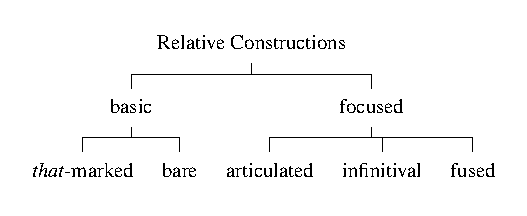
\includegraphics{figures/relative-types.pdf}
    \caption{The syntactic types of relative constructions.}
    \label{fig:relative-construction-types}
\end{figure}

\ea \textsc{basic}\label{ex:basic-rel-clause-types}
    \ea[]{\textit{The places \ob that we like\cb~are nearby.}\hfill[\textsc{\textit{that}-marked}]}
    \ex[]{\textit{The places \ob we like\cb~are nearby.}\hfill[\textsc{bare}]}
    \z
\z
\ea \textsc{focused}\label{ex:focused-rel-clause-types}
    \ea[]{\textit{The places \ob where we study\cb~are nearby.}\hfill[\textsc{articulated}]}
    \ex[]{\textit{They're places \ob in which to study\cb.}\hfill[\textsc{infinitival}]}
    \ex[]{\textit{\ob Where we go\cb~ is nearby.}\hfill[\textsc{fused}]}
    \z
\z

\subsection{Focused types: articulated}\label{sec:focused-articulated}
\is{articulated relative|(}\is{relative word|(}\is{pied-piping}\is{preposition, preposition phrase (PP)!fronting with \textit{wh}- (pied-piping)}\is{register!variation!news/academic}

Articulated relatives are very common, especially in news and academic prose \citep[610 \& 611]{Biber1999}. In many ways they are similar to focused (main-clause) interrogatives. For one thing, focused relatives have a relative word, mirroring the interrogative words of focused interrogatives. These two sets of words overlap significantly. The most important of the relative words are \textit{who}, \textit{whom}\is{whom@\textit{whom}}, \textit{whose}, \textit{which}, \textit{where}, and \textit{when}, along with \textit{why} and \textit{while}, which are less common.  Other minor members include \textit{whence} along with \textit{whereby}, \textit{wherein}, \textit{whereupon}, etc. For comparisons, see Table \ref{tab:interrogative-relative}.
\is{relative word}

\begin{table}[ht]
\centering
\caption{Comparison of Interrogative and Relative Words}
\label{tab:interrogative-relative}
\begin{tabular}{lll}
\toprule
\textbf{Interrogative} & \textbf{Relative} & \textbf{Lexical Category} \\
\midrule
\textit{who}  & \textit{who}  & Pronoun \\
\textit{whom} & \textit{whom} & Pronoun \\
\textit{whose}& \textit{whose}& Pronoun \\
\textit{which}& \textit{which}& Determinative \\
\textit{where}& \textit{where}& Preposition \\
\textit{when} & \textit{when} & Preposition \\
              & \textit{while}& Preposition \\
\textit{why}  & \textit{why}  & Adverb \\
\textit{how}  &    & Adverb  \\
\textit{how}  &    &  Adjective \\
\textit{what} &  \textit{what}\textsuperscript{\dagger}   & Determinative \\
\bottomrule
\end{tabular}\\
\textsuperscript{\dagger}\textit{What} is limited to fused relatives.
\end{table}

Examples of each of relative words appear in (\ref{ex:articulated-relative-words}).

\ea \label{ex:articulated-relative-words}
    \ea[]{\textit{That's the guard \ob \uline{who} \uline{\phantom{he}} we gave it to \cb.}}
    \ex[]{\textit{That's the guard \ob to \uline{whom} we gave it \uline{\phantom{he}} \cb.}}
    \ex[]{\textit{That's the jerk \ob \uline{whose} dog \uline{\phantom{he}} bit me \cb.}\hfill[\textsc{dependent possessive}]}
    \ex[*]{\textit{That's the jerk \ob \uline{whose} \uline{\phantom{he}} bit me \cb.}\hfill[\textsc{independent possessive}]}
    \ex[]{\textit{That's the one \ob \uline{which} I bought \uline{\phantom{it}} \cb.}}
    \ex[]{\textit{That's the place \ob \uline{where} I put it \uline{\phantom{it}} \cb.}}
    \ex[]{\textit{That's the year \ob \uline{when} I was born \uline{\phantom{it}} \cb.}}
    \ex[]{\textit{That's the time \ob \uline{while} I was away \uline{\phantom{it}} \cb.}}
    \ex[]{\textit{That's the reason \ob \uline{why} I did it \uline{\phantom{he}} \cb.}}
    \ex[*]{\textit{That's the way \ob \uline{how} I did it \uline{\phantom{he}} \cb.}}
    \ex[*]{\textit{That's the thing \ob \uline{what} I saw \uline{\phantom{he}} \cb.}}
    \ex[]{\textit{That's \ob \uline{what} I saw \uline{\phantom{he}} \cb.}}
    \z
\z
\is{genitive!dependent vs independent}\is{preposition stranding}\is{relative word|)}

Semantically, the relative words are similar to the interrogatives, except that they refer. Relative \textit{while} denotes durations of time, and \textit{why} is strictly limited to reasons. And although interrogative \textit{whose} is limited to denoting persons, relative \textit{whose} may refer to non-persons as well, as (\ref{ex:whose-non-personal}) demonstrates.\is{relative word!\textit{whose} with non-human antecedent}

\begin{samepage}
    \ea\label{ex:whose-non-personal}
        \ea[]{\textit{I read it in a \uline{book} \ob\uline{whose} title I no longer remember \cb.}\hfill[\textit{relative}]}
        \ex[*]{\textit{Whose title do you no longer remember, the book's?}\hfill[\textit{interrogative}]}
        \z
    \z
\end{samepage}

As with focused interrogatives Section \ref{sec:interrogative-phrases}, focused relative clauses involve fronted phrases (from single words to longer phrases) that leave gaps in their original positions.\is{fronting}\is{movement (fronting)} In articulated relatives, this creates a three-way relationship between the antecedent, fronted phrase, and gap, as shown in \ref{ex:relatives-visualized}.  (\ref{ex:relatives-visualized}) should help you to visualize this situation.

The typical case, with the relative phrase consisting of the relative word alone, is (\ref{ex:relatives-visualized}a). Those like (b--d), where the relative word is a dependent in the relative phrase, are less common.

And, to reiterate, the gaps may be in subject, object, complement, or adjunct positions, as in (\ref{ex:articulated-gap-positions}).

\subsection{Difficulty and syntactic functions} \label{sec:difficulty-relatives}
\is{processing limitations|(}\is{frequency!effect of}\is{subject (Subj)!gap vs object gap}\is{distance effects (antecedent–gap)}

Not all kinds of relative clause are equally easy. This seems to be related to how frequently they appear \citep{Reali2007}, though a clause that is more difficult to process will likely be produced less and so it's hard to say which way the causality goes, or even whether the cause might lie elsewhere. Nevertheless, we can generally say that relative clauses with subject gaps are easier to process than those with object gaps \citep{Lau2021}, as shown in (\ref{ex:teacher-student-liking}).

\ea \label{ex:relatives-visualized}
    \setstretch{2}  % This sets the line spacing to double.
    \ea[]{\textit{I know the \tikzmarknode{a}{\textcolor{xGreen}{place}} \ob\tikzmarknode{A}{\uline{\textcolor{xGreen}{where}}} he works \tikzmarknode{B}{\uline{\phantom{XXX}}} \cb.}}
    \ex[]{\textit{She hasn't yet met the \tikzmarknode{b}{\textcolor{xGreen}{people}} \ob\tikzmarknode{C}{\uline{\textcolor{xGreen}{\tikzmarknode{e}{whose}} house}} she's renting \tikzmarknode{D}{\uline{\phantom{XXX}}} \cb.}}
    \ex[]{\textit{This is the \tikzmarknode{c}{\textcolor{xGreen}{professor}} \ob\tikzmarknode{E}{\uline{to \textcolor{xGreen}{whom}}} I sent it \tikzmarknode{F}{\uline{\phantom{XXX}}} \cb.}}
    \ex[]{\textit{He set them a \tikzmarknode{d}{\textcolor{xGreen}{problem}}, \ob\tikzmarknode{G}{\uline{the an\tikzmarknode{f}wer to \textcolor{xGreen}{which}}} they found \tikzmarknode{H}{\uline{\phantom{XXX}}} \cb~online.}}
    \z
\z

\begin{tikzpicture}[overlay, remember picture]
\draw[-] (A.south) to [bend right=20] (B.south);
\draw[-] (a.north) to [bend left=20] (A.north);
\draw[-] (C.south) to [bend right=20] (D.south);
\draw[-] (b.north) to [bend left=20] ([xshift=-25pt] e.north);
\draw[-] (E.south) to [bend right=20] (F.south);
\draw[-] (c.north) to [bend left=20] ([xshift=5pt] E.north);
\draw[-] (G.south) to [bend right=20] (H.south);
\draw[-] (d.north) to [bend left=20] ([yshift=3pt] f.north);
\end{tikzpicture}

\ea \label{ex:teacher-student-liking}
    \ea[]{\textit{The teacher \ob who \uline{\phantom{it}} liked the students\cb~ marked the tests.}\hfill[\textsc{subject}]}
    \ex[]{\textit{The teacher \ob who the students liked \uline{\phantom{it}} \cb~ marked the tests.}\hfill[\textsc{object}]}
    \z
\z

This recalls the discussion of information packaging (Ch. \ref{ch:info-package}), in particular the section on passive constructions (Section \ref{sec:passive}).\is{information packaging!relative clauses}\is{passive!information packaging} There, we saw that the passive can be used to keep related items together. This could mean keeping the head noun of a subject NP close to the VP, or it could mean fronting a topic so that it is closer to a previous mention. When it comes to relative clauses, those with a subject gap will similarly minimize the distance between the gap and its antecedent.

But there's also the factor of whether or not there are multiple agents. For example, in (\ref{ex:teacher-student-liking}), someone could plausibly misunderstand the direction of liking. In (\ref{ex:articulated-gap-positions}), though, there's only the kid who could be an arriver and one possible raiser, putter, or winner, which simplifies things.

In terms of which NP the relative clause appears in, it seems that a relative clause occurring at the end of the clause is easier to process than one in the middle. This means that a relative in the subject is going to be a bit harder than one in the object. This gives us the illustrative difficulty matrices in Tables \ref{tab:difficulty-matrix} and \ref{tab:difficulty-matrix2}, with 1 being easiest and 4 being hardest, though these numbers are to be interpreted very roughly.
\is{processing limitations|)}

\begin{table}[ht]
\centering
\begin{tabular}{lcc}
\toprule
 & \textbf{Subject gap} & \textbf{Object gap} \\ 
\midrule
\textbf{Relative in subject NP} & 2   & 3 \\ 
\textbf{Relative in object NP}   & 1   & 2     \\ 
\bottomrule
\end{tabular}
\caption{Difficulty matrix for relative clauses with one agent}
\label{tab:difficulty-matrix}
\end{table}

\begin{table}[ht]
\centering
\begin{tabular}{lcc}
\toprule
 & \textbf{Subject gap} & \textbf{Object gap} \\ 
\midrule
\textbf{Relative in subject NP} & 3   & 4 \\ 
\textbf{Relative in object NP}   & 2   & 3     \\ 
\bottomrule
\end{tabular}
\caption{Difficulty matrix for relative clauses with multiple agents}
\label{tab:difficulty-matrix2}
\end{table}

\subsection{Basic types}
\is{that relative@\textit{that}-relative clause|(}\is{bare relative|(}\is{subordinator!\textit{that} (relative)}

In the basic types~-- \textit{that}-marked and bare~-- you get examples like (\ref{ex:basic-relatives}), with the same range of possible gaps as you find in the focused relatives.

\begin{samepage}
\ea \label{ex:basic-relatives}
    \ea[]{\textit{That's the kid \ob that \uline{\phantom{he}} arrived yesterday \cb.}\hfill[\textsc{subject}]}
    \ex[]{\textit{That's the one \ob\op that\cp~I bought \uline{\phantom{it}} \cb.}\hfill[\textsc{object}]}
    \ex[]{\textit{That's the place \ob\op that\cp~I put it \uline{\phantom{it}} \cb.}\hfill[\textsc{complement}]}
    \ex[]{\textit{That's the year \ob\op that\cp~I was born \uline{\phantom{it}} \cb.}\hfill[\textsc{adjunct}]}
    \z
\z
\end{samepage}

When there's a gap in the subject position, as in (\ref{ex:basic-relatives}a), then \textit{that} is obligatory.\\is{that relative@\textit{that}-relative clause!obligatory with subject gap} Otherwise, it's usually optional, as in (b--d). In other words, you have more or less free choice between the \textit{that}-marked and bare types when the gap is in the object (b), other-complement (c), or adjunct (d) positions.\is{bare relative!distribution}

The \textit{that} in \textit{that}-marked relatives is the same subordinator you find in declarative subordinate clauses, such as (\ref{ex:subordinator-that}).\is{subordinator!\textit{that} (declarative vs relative)}

\ea \label{ex:subordinator-that}
    \ea[]{\textit{The idea \ob \op that\cp~ I might be suitable\cb~ was pleasant.}\hfill[\textsc{content}]}
    \ex[]{\textit{The idea \ob \op that\cp~ I had \uline{\phantom{it}} \cb~was pleasant.}\hfill[\textsc{relative}]}
    \z
\z

\subsubsection*{Restrictions on the basic types}
\is{bare relative!ban with subject gap}\is{pied-piping!blocks basic}

The basic relatives have a more limited distribution than the focused types. As we've seen already, bare relatives can't appear if the gap is in the subject position:

\ea
    \ea[]{\textit{The places \ob that \uline{\phantom{it}} suit us \cb~are nearby.}\hfill[\textsc{\textit{that}-marked}]}
    \ex[*]{\textit{The places \ob~\uline{\phantom{it}} suit us \cb~are nearby.}\hfill[\textsc{bare}]}
    \z
\z

If the relative word in the articulated type is a dependent in the relative phrase, neither basic type is possible.

\ea
    \ea[]{\textit{The places \ob \uline{to which} we go \uline{\phantom{it}} \cb~are nearby.}\hfill[\textsc{articulated}]}
    \ex[*]{\textit{The places \ob \op that\cp~\uline{to~~~} we go \uline{\phantom{it}} \cb~are nearby.}\hfill[\textsc{basic}]}
    \z
\z
\ea
    \ea[]{\textit{The friend \ob \uline{whose bike} we borrowed \uline{\phantom{it}} \cb~is nearby.}\hfill[\textsc{articulated}]}
    \ex[*]{\textit{The friend \ob \op that\cp~\uline{bike} we borrowed \uline{\phantom{it}} \cb~is nearby.}\hfill[\textsc{basic}]}
    \z
\z

Also, if the relative clause is in an NP with \textit{that} as its head, the basic types don't work.

\ea
    \ea[]{\textit{That \ob which we like \uline{\phantom{it}} \cb~is nearby.}\hfill[\textsc{articulated}]}
    \ex[*]{\textit{That \ob \op that\cp~we like \uline{\phantom{it}} \cb~is nearby.}\hfill[\textsc{basic}]}
    \z
\z

Another tendency is that basic relatives are quite uncommon after coordinators.

\ea
    \ea[]{\textit{We saw a car \ob which we recognized \uline{\phantom{it}} but which we didn't expect \cb.}\hfill[\textsc{articulated}]}
    \ex[\textsuperscript{?}]{\textit{We saw a car \ob that we recognized \uline{\phantom{it}} but that we didn't expect \cb.}\hfill[\textsc{basic}]}
    \z
\z

Finally, if the relative clause is a supplement, rather than a modifier, the basic types are not possible. A supplemental relative clause is set off in writing with commas and in speech with its own intonation contour.\is{comma!with relative clause}

\ea
    \ea[]{\textit{A jerk, \ob which I am not \uline{\phantom{it}} \cb, would have left.}\hfill[\textsc{articulated}]}
    \ex[*]{\textit{A jerk, \ob \op that\cp~I am not \uline{\phantom{it}} \cb, would have left.}\hfill[\textsc{basic}]}
    \z
\z
\is{that relative@\textit{that}-relative clause|)}\is{bare relative|)}\is{articulated relative|)}

\section{Semantic restriction}
\is{relative clause!restrictive vs non-restrictive|(}\is{semantics!restrictive modifier}\is{semantics!supplement (non-restrictive)}\is{modification, modifier!integrated vs supplementary}

This brings us back to the oft-cited distinction we opened with between `restrictive' vs `non-restrictive'. A relative clause syntactically integrated into the NP as a modifier very often is semantically restrictive. In other words, it tends to identify a subset of the whole set. For example, if there are four books, two of which cover grammar, I can ask, \textit{Can I have the books \ob that}/\textit{which cover grammar}], splitting the whole set of books into those that cover grammar and those that don't. And the response might be (\ref{ex:restrictive-books}).

\ea[]{\textit{The books \ob that}/\textit{which \uline{\phantom{it}} cover grammar \cb~are there.}\hfill[\textsc{restrictive}]}\label{ex:restrictive-books}
\z

It's also true that supplementary relatives are semantically non-restrictive. But if the response were instead (\ref{ex:non-restrictive-books}), it would refer to all of the books, without restriction. The fact that they cover grammar is merely a supplementary fact. 

\ea[]{\textit{The books, \ob which \uline{\phantom{it}} cover grammar \cb, are there.}\hfill[\textsc{non-restrictive}]}\label{ex:non-restrictive-books}
\z

Unfortunately, the common idea that restrictive relatives use \textit{that} and non-restrictive \textit{which}, misses the possibility of focused relatives as modifiers and ignores bare relatives and all the other relative words.

\ea
\ea[]{\textit{A decision \ob everyone likes \uline{\phantom{it}} \cb is hard to make.}\hfill[\textsc{restrictive}]}
\ex[]{\textit{A decision, \ob which we need \uline{\phantom{it}} \cb, is lacking.}\hfill[\textsc{non-restrictive}]}
\z
\z
\ea
\ea[]{\textit{The kids \ob who \uline{\phantom{it}} were abroad{\cb} were successful.}\hfill[\textsc{restrictive}]}
\ex[]{\textit{The kids, \ob who \uline{\phantom{it}} were aboard{\cb}, were successful.}\hfill[\textsc{non-restrictive}]}
\z
\z

Perhaps the most important point is that \textsc{restrictive} and \textsc{non-restrictive} are not clause types but rather descriptions of the semantic force clauses have in different functions: modifier, in the restrictive cases, and supplement, in the non-restrictive cases. The correct generalization is that integrated modifiers tend to be restrictive and supplementary modifiers are not, and only articulated focused relatives may be supplementary modifiers.

And this applies not just to relative clauses. Consider the difference between the (a) and (b) examples in  (\ref{ex:trust-with-integrity} \& \ref{ex:sleepy-guests}).

\ea \label{ex:trust-with-integrity}
    \ea[]{\textit{The kids {\ob}abroad{\cb} were successful.}\hfill[\textsc{restrictive}]}
    \ex[]{\textit{The kids, {\ob}abroad{\cb}}, were successful\hfill[\textsc{non-restrictive}]}
    \z
\z
\ea \label{ex:sleepy-guests}
    \ea[]{\textit{\ob The sleepy and full guests\cb~left, but other guests stayed.}\hfill[\textsc{restr}]}
    \ex[\textsuperscript{?}]{\textit{\ob Sleepy and full\cb, the guests left, but other guests stayed.}\hfill[\textsc{non-restr}]}
    \z
\z
\is{relative clause!restrictive vs non-restrictive|)}

In (\ref{ex:trust-with-integrity}a), the PP \textit{with integrity} is a modifier in the NP, and it has restrictive semantics, picking out the subset of principled friends. The PP in (b), though, is a supplement; (b) means I trust all my friends, principled or not. Similarly, the \textit{sleepy and full} modifier in (\ref{ex:sleepy-guests}a) restricts the set of guests who went home to the sleepy and full subset, while the supplement in (b) declares all guests sleepy and full, making mention of `other guests'' confusing.

\section{Relative clauses as supplements} \label{sec:rel-clause-supps}
\is{supplementary relative|(}\is{intonation!of supplement}\is{punctuation!of supplement}\is{antecedent!non-NP}\is{relative word!\textit{which} with non-NP antecedent}

As I've mentioned, only the articulated focused relatives function as supplements, and, as supplements, they are set off by commas, dashes, or parentheses in writing and have their own intonation contour in speech.

\ea
    \ea[]{\noindent\textglobrise\phantom{guy who likes books is com}\textglobfall \\
    \textit{A guy who likes books is coming.}}
    \ex[]{\noindent\textglobrise~~~\textglobfall~~~\textglobrise\phantom{o likes Ma} \textglobfall \phantom{, is}\textglobrise \phantom{leav}\textglobfall \\
    \textit{Adam, who likes books, is coming.}}
    \z
\z

Interestingly, when relatives function as supplements, the set of possible antecedents widens. Nouns are still possible, but so, now, are VPs, clauses, AdjPs, PPs, and even AdvPs. With these antecedents, the relative phrase is always \textit{which}.

\ea
    \ea[]{\textit{I like \uline{to make soups}, \ob which \uline{\phantom{it}} is good practice \cb.}\hfill[\textsc{VP}]}
    \ex[]{\textit{\uline{He ran}, \ob which \uline{\phantom{it}} caused problems \cb.}\hfill[\textsc{Clause}]}
    \ex[]{\textit{My \uline{poor} grades, \ob which \uline{\phantom{it}} is putting it kindly \cb, worsened.}\hfill[\textsc{AdjP}]}
    \ex[]{\textit{I left \uline{before 6}, \ob which \uline{\phantom{it}} is early \cb.}\hfill[\textsc{PP}]}
    \ex[]{\textit{She finished \uline{well}, \ob which \uline{\phantom{it}} is how she wanted to finish \cb.}\hfill[\textsc{AdvP}]}
    \z
\z
\is{supplementary relative|)}

\section{Relative clauses in \textit{it}-clefts}
\is{cleft (clause)!it-cleft@\textit{it}-cleft}\is{relative clause!in clefts}\is{disambiguation!cleft vs non-cleft}\is{extraposition}\is{content clause!extraposed subject}

As we saw in Section \ref{sec:clefts}, \textit{it}-clefts include a main clause followed by a relative clause. This can be a basic or articulated relative, and the head noun is stressed (indicated by~\textipa{"}~), as in (\ref{ex:it-cleft}), but such clefts are actually relatively uncommon.

\ea \label{ex:it-cleft}
    \ea[]{\textit{ It was my \textipa{"}friend \ob \op that\cp~we met \uline{\phantom{it}} \cb.}}
    \ex[]{\textit{ It was my \textipa{"}friend \ob who we met \uline{\phantom{it}} \cb.}}
    \z
\z

An \textit{it}-cleft like (\ref{ex:it-cleft}), in which \textit{it} has no referent, can easily be confused with a much more common, similar-looking plain old non-cleft construction with a relative, such as (\ref{ex:non-cleft}), in which \textit{it} refers to something like my lack of cash, or forgetting my password. 

\begin{samepage}
    \ea \label{ex:non-cleft}
        \ea[]{\textit{It was a problem \ob \op that\cp~I had not anticipated \uline{\phantom{it}} \cb.}}
        \ex[]{\textit{It was a problem \ob which I had not anticipated \uline{\phantom{it}} \cb.}}
        \z
    \z
\end{samepage}

Another potential confounder, which we saw in Section \ref{sec:extraposition}, and which, again, is much more common, is an extraposed subject like that in (\ref{ex:non-cleft2}). This is a declarative content clause, not a relative. You can tell because it doesn't have a gap. If you're not sure, try replacing the \textit{that} with \textit{which}, as in (b). If it's an extraposed subject, it won't work.

\ea \label{ex:non-cleft2}
    \ea[]{\textit{It was a problem \ob that more people were now coming\cb.}}
    \ex[*]{\textit{It was a problem \ob which more people were now coming\cb.}}
    \z
\z

\section{Pronoun retention, aka ``resumptive pronouns''}
\is{resumptive pronoun|(}\is{pronoun!retention|(}\is{register!variation!speech vs writing}\is{L1 transfer!Arabic→English relatives}

In Standard English, relative clauses contain a gap, but sometimes, the gap is filled with a pronoun linked anaphorically to the antecedent in the matrix clause. This \textsc{pronoun retention}, also known as a ``resumptive pronoun'', is rare but most common in informal spoken registers. In some languages though, notably Arabic\il{Arabic}, pronoun retention is standard and commonly used. As a result, speakers of these languages tend to retain pronouns in English relative clauses as well.\is{cross-linguistic influence}

Consider the examples in \ref{ex:resumptive-pronouns}, which illustrate this construction.
\ea \label{ex:resumptive-pronouns}
    \ea[*]{\textit{This is the house \ob that I painted \uline{it} yesterday \cb.}}
    \ex[*]{\textit{I have a girlfriend \ob who \uline{she}'s really into jazz \cb.}}
    \ex[*]{\textit{There's the books \ob that I told you about \uline{them} \cb.}}
    \z
\z

In Standard English, the pronouns in italics would be omitted, leaving a gap. But in the non-standard examples in (\ref{ex:resumptive-pronouns}), they are retained, ``resuming'' the reference of the antecedents (\textit{house}, \textit{girlfriend}, \textit{books}).

But even expert users of English sometimes retain pronouns in relative clauses, especially when the gap that would otherwise appear is deeply embedded or where the relative phrase would be more than just the relative word, as in (\ref{ex:resumptive-oblique}).\is{embedding!depth effects} The standard version is in (a), while (b) exhibits retention of genitive \textit{her}.

\ea \label{ex:resumptive-oblique}
    \ea[]{\textit{I met the student \ob \uline{whose essay} the teacher said that she liked \uline{\phantom{her}} \cb.}}
    \ex[\textsuperscript{?}]{\textit{I met the student \ob \uline{who} the teacher said that she liked \uline{her} essay \cb.}}
    \z
\z

The greater acceptability of resumptive pronouns in these contexts may be related to processing difficulty. As we saw in Section \ref{sec:difficulty-relatives}, relative clauses are harder to process when the gap is in a non-subject position and when there is more intervening material between the antecedent and the gap. The resumptive pronoun seems to alleviate some of this processing load by overtly signaling the anaphoric relationship and the function of the gap.

From a pedagogical perspective, it may be helpful for learners who retain pronouns to have the situation explained to them, though gaps may be a difficult concept to explain and to grasp. Still, in academic writing and other formal contexts, gaps are generally expected.

As a teaching tool, though, it may actually be useful to retain the written pronouns but put them in brackets or write them on the board with a different colour to indicate that they are merely placeholders.
\is{pronoun!retention|)}\is{resumptive pronoun|)}

\section{The other focused types}
\subsection{Infinitival}
\is{infinitival!relative|(}\is{relative phrase}\is{subject (Subj)!overt subject banned in infinitival relatives}

There is a rather formal and relatively rare type of infinitival relative clause, which I will refer to as \textsc{focused infinitival relatives}. These are most commonly found as complements of prepositions such as \textit{with}, \textit{in}, and \textit{from}. They are characterized by a relative phrase consisting of a preposition followed most commonly by \textit{which} or \textit{whom}. Consider the examples in \ref{ex:focused-infinitival-relatives}.

\begin{samepage}
    \ea \label{ex:focused-infinitival-relatives}
        \ea[]{\textit{Do you have a key \ob\uline{with which} to open it \uline{\phantom{it}} \cb.}}
        \ex[]{\textit{She is the right person \ob \uline{in whom} to put your trust \uline{\phantom{it}} \cb.}}
        \ex[]{\textit{As a base \ob \uline{from which} to conduct raids \uline{\phantom{it}} \cb, it's perfect.}}
        \z
    \z
\end{samepage}

As these examples illustrate, the focused infinitival relative is an integrated relative (it's a modifier within the NP, not a supplementary relative). The relative phrase (e.g., \textit{with which}, \textit{in whom}) is fronted, just as in other focused relative types. After the fronted relative phrase comes an infinitival VP. Crucially, this VP does not contain an overt subject.

In fact, focused infinitival relatives are subject to two strict structural conditions:
\ea \label{ex:focused-infinitival-restrictions}
    \ea  The relative phrase must consist of a preposition followed by a \textit{wh}-NP.
    \ex  There can be no overt subject in the relative clause.
    \z
\z

Condition (a) rules out examples like *\textit{the question which to answer}, where the relative phrase is a bare \textit{wh}-NP without a preposition. Condition (b) excludes *\textit{the person in whom for us to confide}, where \textit{us} is an overt subject.

Despite these restrictions, the gap in a focused infinitival relative clause can correspond to a variety of syntactic functions, just as in other relative clause types. In (\ref{ex:focused-infinitival-relatives}a), for instance, the gap is an adjunct in clause structure. In (b), it's a complement in the \textit{put} VP. And in (c), it's again an adjunct in clause structure.

Given their highly formal flavor and structural complexity, focused infinitival relatives are even rarer than the infinitival relatives we looked at in the previous section. They are unlikely to be a priority for most English language learners. However, for learners aiming at a very high level of proficiency, especially in formal written registers, an awareness of this construction is part of a comprehensive understanding of English relative clauses.

For the language teacher, the main points to note about focused infinitival relatives are:

\begin{enumerate}[noitemsep]
    \item They involve a fronted relative phrase consisting of a preposition + \textit{wh}-NP.
    \item The relative clause has an infinitival VP with no overt subject.
    \item They are always integrated, never supplementary, relatives.
    \item They are restricted to very formal styles.
\end{enumerate}
\is{infinitival!relative|)}

In teaching, focused infinitival relatives are probably best treated as a kind of linguistic curiosity~--  an example of the complex machinery of English relative clauses, but not a construction that learners need to actively master.

\subsection{Fused}
\is{fused relative|(}\is{content clause!interrogative!vs fused relative}

The final type of relative clause construction we have to dig in to is the fused subtype of the focused relative. Like the infinitivals, they're really quite rare and rarely of concern to English-language teachers and learners.

\textsc{Fused relatives} differ from the relative clauses discussed above in that they do not contain a separate antecedent and relative phrase. Instead, these two components are fused into a single constituent. Consider the examples in (\ref{ex:14.11}).

\ea \label{ex:14.11}
    \ea[]{\textit{\ob\uline{Whoever} \uline{\phantom{it}} said that\cb~was mistaken.}}
    \ex[]{\textit{I've heard \ob\textit{\uline{what} you said \uline{\phantom{it}}} \cb.}}
    \ex[]{\textit{\ob\uline{Whichever colour} you pick \uline{\phantom{it}} \cb~will work.}}
    \z
\z

The bracketed portions in these examples are not simply relative clauses, but rather full NPs containing fused relatives. In each case, the underlined relative phrase (\textit{whoever}, \textit{what}, \textit{whichever colour}) simultaneously functions as the antecedent and the relative phrase.

In (\ref{ex:14.11}a), \textit{whoever} is both the head of the NP (comparable to \textit{the person}) and the relative phrase in the relative clause. Similarly, in (\ref{ex:14.11}b), \textit{what} serves as the head of the object NP and the relative phrase in the relative clause. And, in (\ref{ex:14.11}c), the NP \textit{whichever colour} is both the antecedent and the relative phrase.

The relative words used in fused relatives differ somewhat from those used in regular relative clauses. (\ref{ex:14.12}) shows those that appear in fused relatives. 

\ea \textit{whoever}, \textit{whomever}, \textit{whatever}, \textit{whichever}, \textit{wherever}, \textit{whenever}, \\\textit{what}, \textit{where}, \textit{when}, \textit{why}\label{ex:14.12}
\z

Notably, the compound \textit{--ever} words are not just possible but common in fused relatives. \textit{What} is also possible, but \textit{while} is not. 

A potential challenge to the teacher is distinguishing fused relatives from embedded interrogative clauses, which can have a similar surface appearance:
\ea \label{ex:14.14}
    \ea[]{\textit{I'll read \ob what you suggest \uline{\phantom{it}} \cb.}\hfill[\textsc{relative}]}
    \ex[]{\textit{I wonder \ob what you suggest \uline{\phantom{it}} \cb.}\hfill[\textsc{interrogative}]}
    \z
\z

The distinction is not always immediately apparent, but there are tests that can help. For instance, only relative words include the compound \textit{--ever} forms. Compare \textit{I'll read whatever you suggest} and *\textit{I wonder whatever you suggest}.

The reason teachers may need to be aware is so that they do not present a fused relative when they intend to discuss an interrogative. Students, though, should never be asked to distinguish between them, as long as there is no difficulty understanding and producing such examples.
\is{fused relative|)}

\section{Recursive embedding}
\is{recursion}\is{embedding!relative}\is{processing limitations!and recursion}\is{style!complexity vs clarity}

One of the most interesting features of languages like English is \textsc{recursion}~-- the ability to embed structures inside structures of the same type, creating an expandable system from a finite set of rules. Relative clauses provide a prime example of this phenomenon.

Consider the examples in (\ref{ex:recursive-relatives}).
\ea \label{ex:recursive-relatives}
    \ea[]{\textit{This is the cat \ob that \uline{\phantom{it}} killed the rat \textcolor{xGreen}{\ob}that \uline{\phantom{it}} ate the malt \textcolor{xOrange}{\ob}that \uline{\phantom{it}} lay in the house \textcolor{xPink}{\ob}that Jack built \uline{\phantom{it}} \textcolor{xPink}{\cb\textsubscript{4}} \textcolor{xOrange}{\cb\textsubscript{3}} \textcolor{xGreen}{\cb\textsubscript{2}} \cb\textsubscript{1}.}}
    \ex[]{\textit{The book \ob that I borrowed \uline{\phantom{it}} from the library \textcolor{xGreen}{\ob}that \uline{\phantom{it}} is located in the city \textcolor{xPink}{\ob}where I live \uline{\phantom{it}} \textcolor{xPink}{\cb\textsubscript{3}} \textcolor{xGreen}{\cb\textsubscript{2}} \cb\textsubscript{1}~is overdue.}}
    \z
\z

In each of these (slightly whimsical) examples, we have a relative clause that contains within it another relative clause, which may in turn contain yet another, and so on. In (\ref{ex:recursive-relatives}a), for instance, we have four levels of embedding, each introduced by \textit{that}. The subscript numbers indicate the level of embedding, with 1 being the topmost level.

Perhaps, there is no grammatical upper limit on the number of relative clauses that can be nested in this way. Each relative clause is a modifier of the noun phrase that immediately contains it, and any noun phrase can be modified by a relative clause. So the rules of English grammar seem to allow for structures of arbitrary complexity.

However, in practice, there are significant constraints on recursive embedding. The most obvious is the limit of human processing capacity. As the depth of embedding increases, the sentence becomes increasingly difficult to parse and understand. Even for native speakers, more than three or four levels of embedding can start to strain comprehension, especially in spoken language where the hearer doesn't have the luxury of backtracking.

Additionally, highly complex structures like those in (\ref{ex:recursive-relatives}), while grammatical, are often stylistically dispreferred. In most communicative contexts, simpler structures are more effective. Recursive embedding is most commonly found in written, particularly literary, language, where the writer has more time to craft complex structures and the reader has more time to decipher them.

As a teacher, it's probably not necessary to actively teach or encourage deep embedding. But it's useful to be aware of the phenomenon, both to understand the power of the linguistic system and to help learners decipher complex relative clause structures when they encounter them. It can also be used as a kind of add-on game, where each subsequent participant adds another layer.

One practical tip is to encourage learners to break down complex sentences into smaller parts. For instance, (\ref{ex:recursive-relatives}c) could be analyzed as follows:

\begin{enumerate}[noitemsep]
    \item The book is overdue.
    \item I borrowed the book from the library.
    \item The library is located in the city.
    \item I live in the city.
\end{enumerate}

By unpacking the nested structure in this way, the meaning should become clearer.

\section{Phrase Structure}
\is{syntax tree}\is{co-indexing!gap}\is{NP!modifier position for relatives}

Having looked at the main types of relative clauses and their properties, I'll present some trees to explain their structure. As we've seen before, the x subscript (e.g., NP\textsubscript{x}) indicates an anaphoric relationship.

\subsection{Structural types}
\subsubsection*{Basic relatives}
\is{that relative@\textit{that}-relative clause}\is{bare relative!tree}

The following trees show the two basic relative types: bare and \textit{that}-marked. Bare clauses (Figure \ref{fig:we-met}) are not possible with a subject gap, but for the \textit{that}-marked, I've included one with an object gap and one with a subject gap (Figure \ref{fig:that-met-us}).

\begin{figure}[ht]
    \centering
    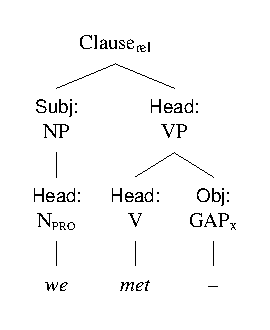
\includegraphics{figures/we-met.pdf}
    \caption{A tree diagram for a bare relative clause in \textit{He's the man we met.}}
    \label{fig:we-met}
\end{figure}

\begin{figure}[ht]
    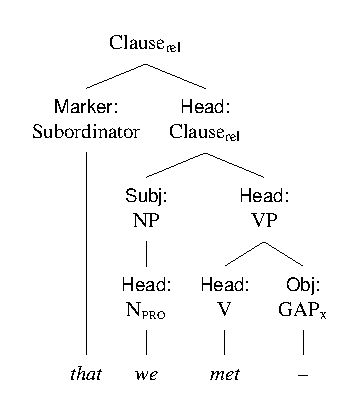
\includegraphics{figures/that-we-met.pdf}
    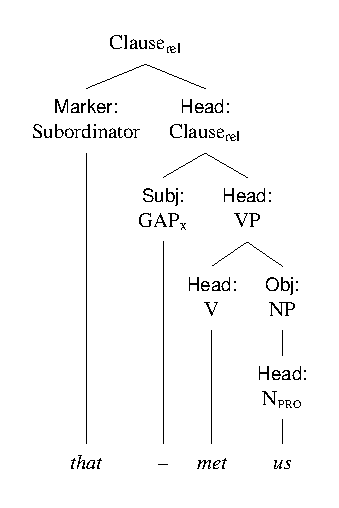
\includegraphics{figures/that-met-us.pdf}
    \caption{Tree diagrams for a \textit{that}-marked relative clauses following \textit{He's the man} with object and subject gaps}
    \label{fig:that-met-us}
\end{figure}

\newpage
\subsubsection*{Focused relatives}
\is{articulated relative!tree}\is{infinitival!relative!tree}\is{fused relative!tree}

The next set of tree diagrams shows the focused types. There are three articulated relatives: a pair with object and subject gaps (Figure \ref{fig:who-met-us}) and one with a complex relative phrase (Figure \ref{fig:whose-title-I}). These are followed by a tree showing the structure of the infinitival subtype (Figure \ref{fig:in-whom-to-trust}) and one for the fused subtype (Figure \ref{fig:whoever-you-suggest}).

\begin{figure}[ht]
    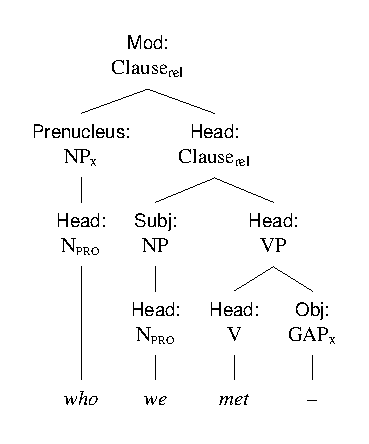
\includegraphics{figures/who-we-met.pdf}
    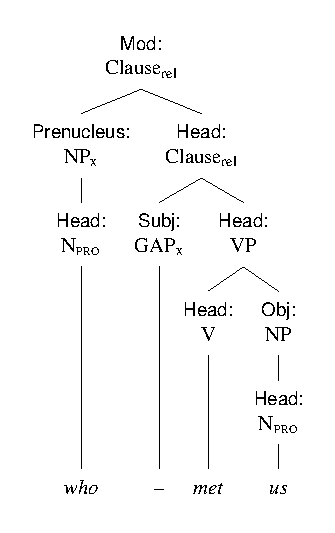
\includegraphics{figures/who-met-us.pdf}
    \caption{Tree diagrams for articulated relative clauses with object and subject gaps}
    \label{fig:who-met-us}
\end{figure}

\begin{figure}[ht]
    \centering
    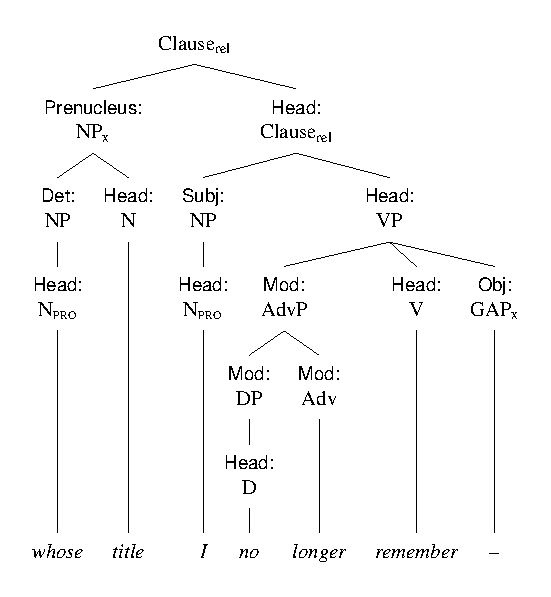
\includegraphics{figures/whose-title-I-no-longer-remember.pdf}
    \caption{A tree diagram for an articulated relative with a complex relative phrase.}
    \label{fig:whose-title-I}
\end{figure}

\begin{figure}[ht]
    \centering
    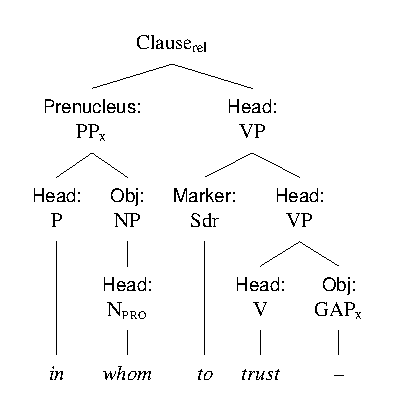
\includegraphics{figures/in-whom-to-trust.pdf}
    \caption{A tree diagram for an infinitival relative.}
    \label{fig:in-whom-to-trust}
\end{figure}

\begin{figure}[ht]
    \centering
    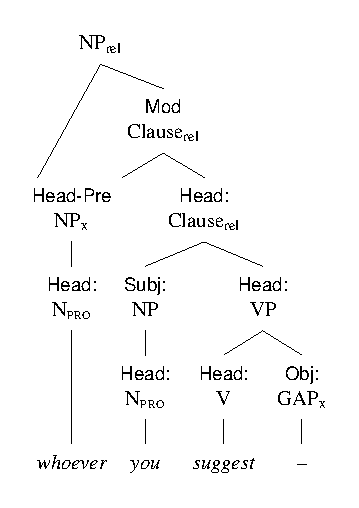
\includegraphics{figures/whoever-you-suggest.pdf}
    \caption{A tree diagram for a fused relative.}
    \label{fig:whoever-you-suggest}
\end{figure}

The structure in Figure \ref{fig:whoever-you-suggest} has a new function label: \textsf{Head-Pre}. This denotes the fusion of the head function of the NP and the pre function. In other words, it shows that \textit{whoever} is both the head of the NP and simultaneously a pre in the relative clause. The fusion is also indicated by the two branches coming to the single word, first branch coming from the NP and the second from the relative clause.\is{function, syntactic!labels in trees!Head-Pre}

\subsection{Relative clauses as modifiers in NP structure}
\is{modification, modifier!post-head}\is{co-indexing!gap}

Most relative clauses function as modifiers in NP structure, appearing after the head noun, as in Figure \ref{fig:the-places-we-saw}. This is no different than any other post-head modifier.

\begin{figure}[ht]
    \centering
    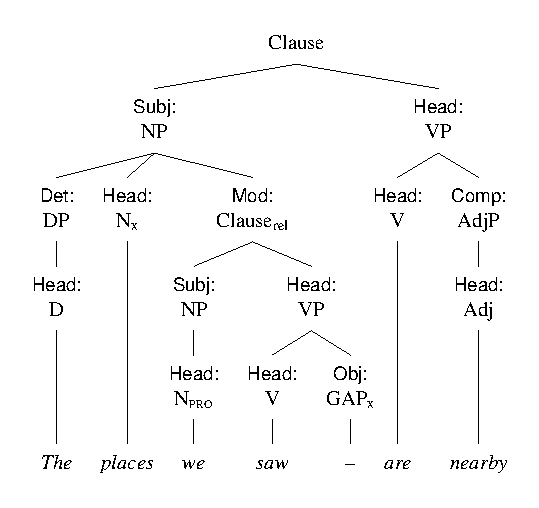
\includegraphics{figures/the-places-we-saw.pdf}
    \caption{A tree diagram for a relative clause as a modifier in NP structure.}
    \label{fig:the-places-we-saw}
\end{figure}

A small difference here is that, because it's a bare relative, the GAP\textsubscript{x} is co-indexed not with the relative phrase, because there isn't one, but with the head noun in the NP, in this case, \textit{places}.

\subsection{Supplementary Relative Clauses}
\is{supplementary relative!attachment site}\is{clause!supplement}

As Figures \ref{fig:a-guy-who-likes} and \ref{fig:he-ran-which} show, supplementary relative clauses are not integrated into the NP but rather attached as supplements to the main clause. They always involve an articulated relative clause.

\begin{figure}[ht]
    \centering
    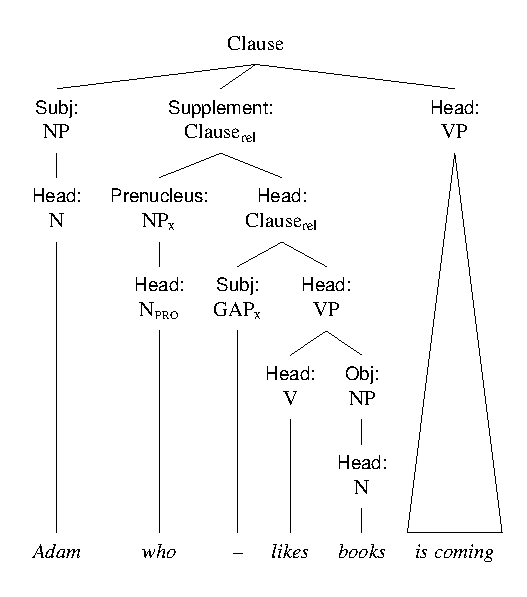
\includegraphics{figures/adam-who-likes-books.pdf}
    \caption{A tree diagram for a relative cause as a supplement in NP structure.}
    \label{fig:a-guy-who-likes}
\end{figure}

\begin{figure}[ht]
    \centering
    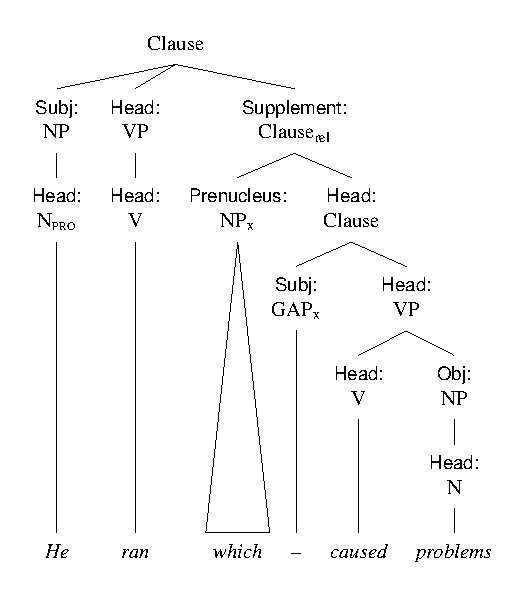
\includegraphics{figures/he-ran-which-caused-problems.pdf}
    \caption{A tree diagram for a relative cause as a supplement in clause structure.}
    \label{fig:he-ran-which}
\end{figure}

\is{supplement vs modifier|)}\is{gap, gapping!in relative clauses|)}\is{relative clause!focused|)}\is{relative clause!basic|)}\is{relative clause|)}\is{relative construction|)}\is{relative clause!bare}
